
\section{BUSINESS ASTROLOGY AND FINANCES IN CHART ANALYSIS}
 

In this lesson we will concentrate on one of the more important aspects of outer chart interpretation, finances and income from career. These indications extend to Mundane Astrology that will be examined in greater detail in Part III of the course and are not simply limited to the birth chart.

 

Vedic Astrology stresses spiritual rather than commercial values. Its concern is not in promoting our ego desires but our souls aspirations. Yet Vedic Astrology does recognize the need to provide for our livelihood. It is also concerned with promoting spiritual and humanitarian activities in the world, which may have a financial or business side to consider. As such, Vedic Astrology does have a business astrology in harmony with its ethics. As Vedic Astrology shows us how to time events for maximum utilization of our resources, it can be used on a business level, but we must make sure we are promoting what is really helpful for the good of all. Vedic Astrology gives us tools not only for insuring the success of business transactions but also for maintaining their spiritual integrity and harmony with the cosmos.

 

It is easier to see the general financial potential in the birth chart and its fluctuations over time through the planetary periods. Using Vedic astrology for timing of investments or even stock market transactions is often done, but it is much more difficult to be accurate with as many of these factors change on a daily basis. There are several factors to consider in judging the appropriate times for business transactions. They are important to consider in the Horary Charts done for business ventures or in selecting appropriate times for business decisions (note the third section of the course in this regard). They can also be used to judge the business acumen or integrity of individuals, through the examination of their birth charts. These connect with general issues of income and career.

 

Personally I have not focused on using astrology for business transactions, but generally it is not difficult to see the basic financial and career potentials of a person through the birth chart, its Dhana or wealth-giving Yogas versus its Daridra or poverty-giving Yogas. This usually involves focusing in the second house of livelihood along with the eleventh and twelfth houses of gain and loss. Fourth house as property, fifth house of investment, ninth house of good fortune and eighth house relative to inheritance come into play here.

We begin with an auto overview of this issue.


\subsection{\textbf{Business, Wealth and Abundance in the Vedic Chart}}

\begin{figure}[H]
 \centering
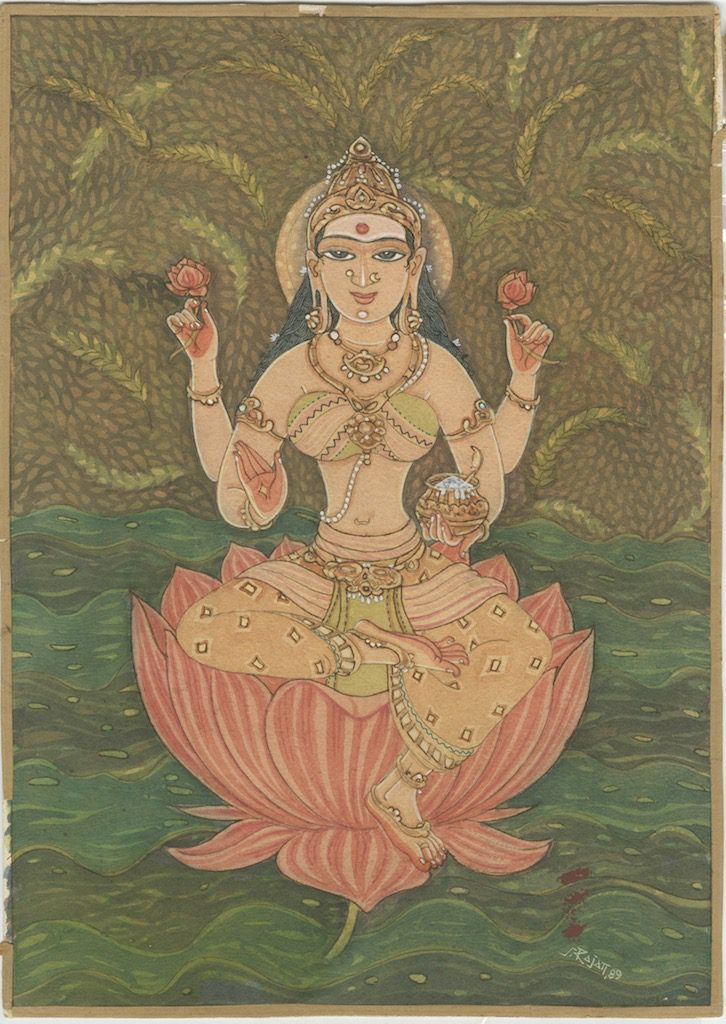
\includegraphics[width=0.8\textwidth]{pics/business1.png}
\caption{Devi Lakshmi who Rules over Wealth and Abundance}
 \end{figure}





 

\subsection{WEALTH INDICATIONS OF THE HOUSES AND THEIR LORDSHIP}
 

Houses of wealth and their lords are most important for income, whether we are considering the birth chart or muhurta (timing charts)

 

\begin{enumerate}
\item[*] The eleventh house and its lord gives good income, particularly that through our friends, associations and greater goals in life.\\
\item[*] The ninth house and its lord gives good luck, the favor of the government or other established authorities.\\
\item[*] The fifth house and its lord gives gain through speculation, like stocks and bonds, or good advice.\\
\item[*] The fourth house and its lord gives gains through property, vehicles and fixed assets.\\
\item[*] The second house and its lord shows gain through our own personal efforts or work we do with our own hands or with our speech.\\
\item[*] The tenth house and its lord gives social recognition, status and prestige.\\
 \end{enumerate}

Houses of poverty and their lords should not be prominent.

 

\begin{enumerate}
\item[*] The twelfth house and its lord gives high expenses and causes loss.
\item[*] The sixth house and its lord gives enmity, legal difficulties and disease.
\item[*] The eighth house and its lord creates obstacles, oppression and alienation.
 \item[*] The tenth house and its lord gives social recognition, status and prestige.\\
 \end{enumerate}

The lords of the third, sixth and eleventh houses can make us aggressive and cause us to act too hastily and without the right foundation. Hence, initial success may be followed by a fall. This is particularly true of the lords of the third and sixth. The lord of the eleventh may give wealth but we may be too impulsive or aggressive in using it and may lack the ethical outlook to make it a positive force in the world.

           

Planets that rule houses of wealth are strong if they are placed in their own signs or exaltation. They are also strong if placed in an angle from the Ascendant or the Moon. The lord of the eleventh in the tenth house is good for income through career. It is additionally good if they have an exchange or association with the Lord of the Ascendant. The lord of the second with the ascendant lord is good for income through ones work.

 

There should be associations or exchanges between the lords of houses of wealth. The lord of the ninth, for example, is good in the eleventh and the lord of the eleventh is good in the ninth. This gives good luck and favor from authorities. The lord of the second in the eleventh is good for income through ones work, as is the lord of the eleventh in the second. The lord of the fifth in the eleventh shows income through stocks or speculative ventures, as does the lord of the eleventh in the fifth. The lord of the fourth in the eleventh is good for property income, as is the lord of the eleventh in the fourth. 

 

There should not be exchanges between the lords of houses of wealth and those of houses of poverty. If the lord of the second is in the twelfth and the lord of the twelfth is in the second, this is a strong yoga for poverty. Similarly, it is not good if the lord of the sixth is in the fifth or the lord of the fifth is in the sixth, or if the lord of the ninth is in the eighth or vice versa.    

 

\subsection{INDICATIONS OF HOUSES FOR FINANCIAL GAIN}

 

Houses that give wealth should be strong, tenanted or aspected by benefics, and their lords should also be strong. Houses that give poverty should be untenanted.
Aspects of separative planets (Sun, Mars, Saturn, Rahu and the lord of the twelfth) should be avoided on houses of wealth, particularly on the tenth house that governs career.
 

\begin{enumerate}
\item[*] Planets in the eleventh give abundance, the realization of our aims and good income.

\item[*] Malefics like Saturn, Mars and the Sun do particularly well here for financial purposes.

\item[*] Benefics in the ninth give good luck, fortune and favor in legal ventures, particularly Jupiter, but malefics are to be avoided here.

\item[*] Benefics in the fifth give gain through stocks and speculative ventures, particularly Jupiter. Malefics here also cause harm.

\item[*] Planets in the fourth give property and vehicles. Saturn here is also good for this.

\item[*] Benefics in the second give good income through our own personal work but malefics can cause difficulty. Both Jupiter and Mercury do well here.

\item[*] Planets in the tenth, benefic or malefic, give us the power to influence the public but Saturn here often raises us up only to take us down again. 
 \end{enumerate}
 

Planets should not be located in houses of loss. Planets in the twelfth will give high expenses. However, if we are engaged in some charitable ventures we may have benefics or well placed planets in the twelfth. We should also note that some people who have both high income and high expenses will have a prominent twelfth house but other strong wealth- giving houses to balance it out. Venus in the twelfth, however, is generally good for wealth. The twelfth as the house of foreign countries can also show material activities in foreign lands, including import/export.

Planets in the eighth also give such financial difficulties. However, in insurance and inheritance matters, well-placed planets here are helpful.

Planets in the sixth give legal difficulties, enmity or conflict.  But well placed planets in the sixth, like Jupiter, Mercury or the Moon are often found in health or service ventures.

 

 



\subsection{THE MOON AND OUTER VENTURES: ISSUES OF TIMING}
 

Now we will examine broader issues of the influence of the Moon on financial ventures, mainly relative to timing, but these factors are helpful to know relative to the birth chart also. The Moon represents our capacity to influence people, to have an impact upon society, to reach the masses or large numbers of people. It gives popularity and recognition and keeps us in harmony with the trends of the time. Hence, for business ventures, particularly those that aim at the public or whose concern is teaching or communication, a strong Moon is necessary.

 

In addition, the Moon governs the birth or the first phase of all ventures. A strong Moon is important for the time of initiating important enterprises. It continues to rule them until they are off the ground (out of the womb as it were).

 

For timing of actions or decisions generally, the Moon should preferably be waxing. Generally, it should be between three days after the new Moon and full. The eleventh day of the Moon is best. The day of the full Moon is also good, preferably before the moment the Moon has exactly reached full.

 

The Moon in cardinal signs is better for starting ventures and provides more initiative and dynamic expression. It is better for ventures that aim at leadership, introducing new ideas or having a strong expression and influencing people. In fixed signs, the Moon is better for giving continuity and endurance to our projects. It is better for long term projects, fixed assets or property. In mutable signs, the Moon functions for reexamination or reformation of projects or working out their details. It is also better for matters involving communication or transaction of commodities and can be helpful for intellectual or artistic ventures.

\subsection{THE MOON IN SIGNS}
 

The Moon should reside in favorable or friendly signs. Cancer and Taurus, its own sign and sign of exaltation, are generally good for all enterprises. Cancer is better for matters involving the public or social influence, affairs of the home or personal communication. Taurus is better for those involving material resources, including articles of luxury such as gemstones.

 

\paragraph{THE MOON IN ARIES} is good for starting new ventures, particularly those dealing with science or the mind. It is good for projects that are inventive and are opening up new ground. It is more a time to develop new ideas, however, than to begin practical actions or to set up shop. It is better for projects promoting oneself or a particular personality. One must beware of being overly impulsive as it is not entirely wise to trust ones instincts at this time. One can be headstrong and too aggressive under its impulse.

 

\paragraph{THE MOON IN TAURUS} is good for artistic ventures or for businesses aiming at comfort and luxury. It is good for business partnership, particularly between husband and wife. It is good for dealing with fixed assets. It is also good for poetry, film and other affairs of Venus.

 

\paragraph{GEMINI MOON} is good for communication, writing and teaching ventures. It is good for educational pursuits, commerce, exchange of ideas, information and commodities generally but it is a fluctuating influence that is not always good for fixed enterprises or starting companies. Nothing should be trusted under its impulse unless it is done in contract.

 

\paragraph{CANCER MOON} is good generally for expressing our ideas and feelings to other people. It is good for healing enterprises, for food or domestic concerns and for influencing others generally and working with the masses. It requires that we are sensitive to public opinion, however.

 

\paragraph{LEO MOON} is good for projecting the power of our personality, for ventures having to do with the projection of our own will, character, fame, influence, status or honor or those of some personality. It gives good P.R. but requires that we take a leadership role. It will draw attention to us personally and we should be ready to deal with that. If afflicted, it can cause some negative notoriety.

 

\paragraph{VIRGO MOON} is good for healing, writing, art, crafts, sports, science and service ventures. It is one of the best Moon positions for getting to the details of practically establishing something. There is some danger of getting too caught in details, however. Hence, it is often better for finalizing rather than making initial decisions in a project. It is better for modest ventures than for great projects and by its mutable disposition may give ups and downs and make it difficult to maintain a long-term venture.

 

\paragraph{LIBRA MOON} is good for artistic, spiritual and political affairs. It is appropriate for new ventures designed to change or reform the world and communicate values of harmony and justice to the masses. It gives diplomacy and the capacity to influence people on a subtle level. There may, however, be a danger of being overly idealistic or fanatical. There may be impracticality, as ideas become more important than actual resources. It is also good for projects relating to Venus, like art.

 

\paragraph{SCORPIO MOON} is generally unfavorable for business matters, as it shows emotional confusion, domination and manipulation. It may cause conflict, emotional entanglement and legal problems. However, if its fall is canceled, it can be good for shamanism, psychology, astrology, religion, poetry, healing and scientific research.   

 

\paragraph{SAGITTARIUS MOON} is good for legal enterprises, for projects with religious groups, for working with governments, or with ones ancestors and their traditions. It gives clarity and order in action. It is good for establishing our principles and values. It is also favorable for travel. It is warm, friendly, expansive and optimistic but can attempt too many things.

 

\paragraph{CAPRICORN MOON} is good for influencing society, for establishing institutions, for working with traditions. It is often political. It gives objectivity and detachment, as well as the capacity to orient material resources. It is a good place to have the Moon to make business decisions, issues of money or property, but may lack in vision or sensitivity to the views of others. It is better for long term ventures or those slow to develop because the influence of Saturn will slow things down but make them strong in the long run. It is good for property and other affairs of Saturn.

 

\paragraph{AQUARIUS MOON} is usually not favorable for outer ventures. It gives faith, renunciation, dependency, and otherworldliness. Well‑placed, it is good for religious and spiritual enterprises and gives a capacity for group action. In this way, it can be good for charities and humanistic work. It is better for following than leading. It may cause us difficulties beyond our control or obstruction from friends or allies. It may indicate unrealistic ideas or expectations or show a venture with an inherent negativity and self-destructiveness. On a lower level, Aquarius Moon may get us involved in underworld dealings, like drugs or other forces of deception and illusion.            

 

\paragraph{PISCES MOON} is good for art, imagination, enthusiasm, and intuitive ventures, as well as for affairs involving the sea or commerce across the sea. It is creative and good for establishing new motivation but lacks in objectivity and consistency. It gets carried away by moods, whims or enthusiasm. Hence, it requires careful scrutiny. It is often too fluctuating to be trusted.

 

When judging the position of the Moon in signs, we should also consider that of the ruler of the sign in which the Moon is located (its dispositor). It should also be favorably placed, particularly relative to the Moon, and be in a friendly relationship to it.

\subsection{ASPECTS TO THE MOON}
 

The Moon should be free as much as possible of unfavorable aspects. Conjunction with Rahu, the north lunar node, creates false imaginations and unrealistic plans. It may get us carried away by unreliable mass trends, or though our business may be successful its spiritual and psychological complications may prove difficult or unwholesome.

 

A little influence of Saturn on the Moon may be good as it gives objectivity, but very much can give negativity, an overly conservative nature and the inability to make use of opportunities. Outwardly it can give obstructions and result in loss.

 

Aspects of Mars to the Moon can cause impulsive or rash action and can show conflict or legal difficulties. Problems of communication with the public may arise. Ketu, the south node, causes contraction and may give difficulties or obstructions beyond our control, including conflict or contradictory situations.

 

The best aspect to the Moon is a good influence of Jupiter. Aspects of Jupiter or Jupiter in an angle from the Moon, particularly if Jupiter is exalted or in its own sign, are good. Jupiter gives expansiveness and success, and usually right values, as well as the favor of legal, business and government influences.

 

Aspects of Mercury aid in proper communication and exchange of information. This is useful in all ventures but particularly affairs of teaching or communication. Mercury in itself, unless it is the ruler of houses of income, however, may not be strong enough to give success.

 

Venus gives charm and ability to influence and is usually helpful in gaining resources for us. Its influence is good for artistic matters or projects involving women.

 

\subsection{THE MOON AS HOUSE LORD}
 

The Moon should be the lord of favorable business houses from the ascendant. Favorable ascendants in which the Moon rules positive houses for business are: Aries (4), Gemini (2), Cancer (1), Virgo (11), Libra (10), Scorpio (9), Capricorn (7), and Pisces (5). If not the lord of good houses, the Moon should be well placed or well aspected to compensate for this.        

 

\begin{enumerate}
\item[*] For Aries ascendant the Moon, as ruler of the fourth house, gives property, domestic or emotional happiness.
\item[*] For Gemini, as ruler of the second, it gives income and gains in ones personal occupation.
\item[*] For Cancer, as ruler of the ascendant, it furthers all enterprises generally and exalts ones personality.
\item[*] For Virgo, as ruler of the eleventh, it gives good income and high values.
\item[*] For Libra, as ruler of the tenth, it gives fame, status and social recognition.
\item[*] For Scorpio, as ruler of the ninth, it gives good luck and favor of government, spiritual or religious groups.
\item[*] For Capricorn, as ruler of the seventh, it gives political and social power and capacity to work with partners.
\item[*] For Pisces, as ruler of the fifth, it gives gain through children, creativity, speculation and good advice.
\item[*] For Taurus, as ruler of the third, the Moon gives energy and curiosity but not always good business sense. The individual may be too impulsive to be successful.
\item[*] For Leo, its function depends upon the planet which most influences it as it is lord of the twelfth. By itself it gives loss.
\item[*] For Sagittarius, it gives capacity for profound thinking but not always practical sense, though it is good for inheritance. Again, its value depends a lot upon how it is influenced as ruler of the eighth which also has a neutrality to it.
\item[*] For Aquarius, it is good for service or healing work, but not so much for income or commercial ventures and may give legal problems, as it is ruler of the sixth.
 \end{enumerate}


\subsection{THE MOON IN HOUSES}
 

In terms of house location, the Moon is best placed in angular or trine houses – 1, 4, 5, 7, 9 & 10 – as these give it strength. The fourth house is the strongest as it has directional strength as well.

 

However, the Moon can also be good if it is located in houses of income like 2, 5, 9 & 11. It is excellent if it is located in angular houses as the lord of a house of income; for example, the Moon in the tenth house as lord of the eleventh, as for Virgo ascendant is very good. It is also good if it is exalted or in its own sign in a house of income; for example, the Moon in Cancer in the eleventh for Virgo ascendant, or the Moon exalted in Taurus in the eleventh for Cancer ascendant.

 


\subsection{JUDGING MOTIVATION}

For integrity in business ventures, the Moon should be associated with the lord of the ninth from the ascendant or with sattvic planets like Jupiter and the Sun. Mercury should similarly have sattvic influences. Mars and Saturn should not be too strong or in association with each other. Combinations of Mars and Venus are also to be avoided as they accentuate the emotional nature.


\subsubsection{OUTER INDICATIONS OF OTHER PLANETS}
Once the Moon is strong and under good influence, it is important to examine the other planets which govern business ventures.

 

\paragraph{MERCURY }

A good Mercury is necessary for the proper communication which all enterprises depend upon. It governs the second stage of ventures, when we are in a position to communicate them to others and do commerce through them. It gives ease in the exchange of commodities and ideas. It is also particularly important for affairs dealing with communication, writing, teaching, and healing.

 

It is better if Mercury is not retrograde, or in conjunction with the lunar nodes (unless in its own sign). Nor should it be within two degrees of the Sun, as this blocks objectivity.

 

Mercury conjunct or aspect Jupiter is very favorable and gives practical gains. Jupiter gives expansiveness and Mercury the ability to influence others through it. Mercury with Venus is good for creative or artistic pursuits. Mercury with Saturn is all right for property or for serious mental pursuits but otherwise not good. It makes one materially conservative. Mercury with Mars is good for scientific or legal ventures but is apt to make one overly aggressive.

 

Mercury should not be debilitated which gives immaturity and foolishness, or at least impracticality. Its better signs for location are Taurus, Gemini, Leo, Virgo, Libra, Capricorn, Aquarius, which are those of its friends. It is better located in houses 1, 2, 4, 5, 7, 9, 10 & 11. Mercury is a very strong wealth-giving planet for Leo ascendant as  it rules two houses of wealth, 2 and 11.

 

\paragraph{JUPITER}

Jupiter is the main planet that gives wealth, hence he should be favorably placed and aspected. Jupiter governs the main phase of any activity, when its greatest expansion and success occurs. It gives optimism, the capacity for action and strong endurance. It is good for all business enterprises particularly where there are legal, government or religious groups to deal with. It is good for all charitable ventures as well.

 

Its better signs are Aries, Cancer, Leo, Scorpio, Sagittarius, Aquarius and Pisces. Jupiter is a strong wealth-giving planet for Aquarius by the dual houses of wealth it rules, 2 and 11. It is better located in houses like that given under Mercury, particularly in its own sign or exalted. Jupiter in air signs is good for knowledge but not always for the holding of wealth.

 

\paragraph{VENUS}

Venus gives the charm and charisma necessary to carry out most ventures relating to the public. It is good for enterprises that depend on quality, taste and high values, rather than mass marketing. It is good for businesses involving women or products aimed at them. It is good for vehicles as well. It is essential for artistic and creative ventures. Venus gives wealth and luxury but not always motivation, the urge to work, willingness to do service or great generosity.

 

\paragraph{SATURN}

Saturn shows the obstacles we have to face in our endeavors. It indicates the time that may be needed to accomplish them. It gives property and enduring status but only after persistent effort and often many ups and downs. It may raise us up but can also bring us down, particularly if our actions are selfish.

 

It is usually not favorable to have Saturn in the tenth house, particularly by itself, in any career venture. It does well in the eleventh, however. It is mainly good for property. A strong Saturn is also helpful for working with the government or other institutions and organizations.

 

\paragraph{MARS}

Mars shows the energy and motivation that we have to accomplish things. Well placed, it gives leadership, decisiveness, dynamism and inventiveness. Misplaced, it can make us reckless or too forceful in our actions and bring us into conflict or legal complications.

 

Mars is better for scientific and technical ventures. It gives logic as well. A strong Mars is good for legal affairs, but may cause us to push things too far.

 

\paragraph{THE SUN}

The Sun shows the power of our will and character we have to rely on, or the authority we are able to create. It gives us honor, respect and prestige and often gives the good grace of the government or whatever powers we are looking up to.

 

It does not do well in the second house, however, as it can show high expenses. Its malefic affect on houses should be considered. It is particularly important for ventures that depend upon a strong force of character and individuality, which require a famous or well recognized personality.

 

\paragraph{RAHU, THE NORTH NODE}

Rahu shows our greatest desires. It indicates our area of greatest success, on one hand, and our area of most unrealistic expectations, on the other. It is usually not to be trusted, though it can be a source of many good ideas that need to be validated by other sources.

 

Well placed, as in the tenth house, it can give great success, particularly with the public, as with mass media ventures or communication projects. It sometimes does this if located in other angles like the seventh and the first. It is usually good for income if placed in the eleventh or for good fortune if placed in the ninth. In the sixth it can be good for success in legal ventures. As usual, we must always consider the strength of its lord and the houses its lord rules.

 

\paragraph{KETU, THE SOUTH NODE }

Ketu shows our hidden resources, our psychic reserve. Yet for outer ventures it causes negativity and doubt. Only with planets in their own or exaltation sign does it become a powerful augmenting force and will tend to magnify whatever influences they possess. Ketu with the lord of the second or eleventh houses in their own sign or exalted is particularly good for wealth. This is especially true if the planet involved is Mercury or Jupiter.

 
\subsection{PLANETARY PERIODS}

 

Once the Moon and the other planets are strong and under good influences, we have to consider the dashas or planetary periods. The planetary periods of the birth or horary charts should be given their proper attention. Even if the chart is good the results cannot be gained if the period is not right for it.

 

We should note the major and minor planetary periods governing the time of the chart. These should be of planets that can give wealth, like Jupiter, Venus or Mercury, or of the rulers of houses of wealth like the second, fifth, ninth and eleventh. Generally, a combination of periods of lords of different houses of wealth is very good. For example, if the major period is of the lord of the tenth house, the minor period of the lord of the second, the subminor the lord of the ninth, it should be very good. If on top of this there is a good transit of Jupiter, the period becomes very strong.

 

Periods of the lord of eleventh house usually give income if well placed. Periods of the lord of the second are favorable for career gains. Periods of the lord of the fourth give property or vehicles. Periods of the lord of the ninth give good fortune, luck or sudden and unexpected gains.

 

Similarly, periods of malefics or malefic lords cause difficulties. The period of the lord of the twelfth house can give loss or high expenses (again consider the other house the planet rules). The period of the lord of the eighth gives adversity. The period of the lord of the sixth gives legal or health difficulties which have financial implications.

 

\subsection{SUMMARY}

 

It is difficult to find a birthchart or horary time that is entirely good for all these factors of wealth and prosperity. It is always the majority of factors that has to be considered. A strong birthchart is always a good foundation to work with and will yield good results over time (though not all the time). Then timing comes into play.

 

Then it is best to consider the length of the time period when a venture should be done. If it has to be started within a three-month period, then we look to the favorable positions available at those times by way of transit and choose the best. We can use astrology, particularly the birthchart, to see if the ventures should be started soon or whether one should wait. This depends upon the birthcharts of the people within the business.